%%%%%%%%%%%%%%%%%%%%%%%%%%%%%%%%%%%%%%%%%%%%%%%%%%%%%%%%%%%%%%%%%%%%%%%%%%%%%%%%%%%%%%%%%%%%%%%%%%%%%%%%%%%%%%%%%%%%%%%%%%%%%%%%%%%%%%%%%%%%%%%%%%%%%%%%%%%%%%%%%%%%%%%%%%%%%%%%%%%%%%%%%%%%%%%%%%%%%%%%%%%%%%%%%%%%%%%%%%%%%%%%%%%%%%%%%%%
%%%%%%%%%%%%%%%%%%%%%%%%%%%%%%%%%%%%%%%%%%%%%%%%%%%%%%%%%%%%%%%%%%%%%%%%%%%%%%%%%%%%%%%%%%%%%%%%%%%%%%%%%%%%%%%%%%%%%%%%%%%%%%%%%%%%%%%%%%%%%%%%%%%%%%%%%%%%%%%%%%%%%%%%%%%%%%%%%%%%%%%%%%%%%%%%%%%%%%%%%%%%%%%%%%%%%%%%%%%%%%%%%%%%%%%%%%%
%%%%%%%%%%%%%%%%%%%%%%%%%%%%%%%%%%%%%%%%%%%%%%%%%%%%%%%%%%%%%%%%%%%%%%%%%%%%%%%%%%%%%%%%%%%%%%%%%%%%%%%%%%%%%%%%%%%%%%%%%%%%%%%%%%%%%%%%%%%%%%%%%%%%%%%%%%%%%%%%%%%%%%%%%%%%%%%%%%%%%%%%%%%%%%%%%%%%%%%%%%%%%%%%%%%%%%%%%%%%%%%%%%%%%%%%%%%
\chapter{Introduction}
\label{ch:Introduction}

The determination and quantification of the quality of the jet transverse momentum measurement is of crucial interest for many analyses with jet final states, 
\eg the measurement of the dijet cross section~\cite{bib:CMS:QCD_measurements} or $\ttbar$ production cross sections \cite{bib:CMS:TopCrossSection_8TeV}. 
Also searches for physics beyond the standard model with missing transverse momentum (\PTm) in the final state need a good knowledge of \PTm originating from wrongly measured jets \cite{}.
For analyses relying on information from simulation it is very important to correct the simulated resolution to the resolution actually present in data.
Therefore, scale factors will be presented to adjust the resolution in simulation to the resolution of the real detector.  
  
In the following sections, a data-based method to measure the jet \pt resolution in $\GAMJET$ events will be presented. 
A similar method was already accomplished in earlier analyses \cite{bib:CMS:JERCPaper_2011,bib:CMS-AN-2010-076,bib:CMS-AN-2010-141,bib:CMS-AN-2011-004} of 7\tev data.  
It is further developed here and applied to 8\tev data.

The method is based on the transverse momentum balance in the $\GAMJET$ system. 
It takes advantage of the high resolution of the electromagnetic calorimeter and hence the excellent measurement of the photon energy.
Without initial and final state radiation, the photon and the jet are balanced in the transverse plane. 
Thus, measuring the photon \pt with high accuracy leads to an estimate of the true jet transverse momentum offering a possibility to quantify the resolution of jet \pt measurements.


%%%%%%%%%%%%%%%%%%%%%%%%%%%%%%%%%%%%%%%%%%%%%%%%%%%%%%%%%%%%%%%%%%%%%%%%%%%%%%%%%%%%%%%%%%%%%%%%%%%%%%%%%%%%%%%%%%%%%%%%%%%%%%%%%%%%%%%%%%%%%%%%%%%%%%%%%%%%%%%%%%%%%%%%%%%%%%%%%%%%%%%%%%%%%%%%%%%%%%%%%%%%%%%%%%%%%%%%%%%%%%%%%%%%%%%%%%%
%%%%%%%%%%%%%%%%%%%%%%%%%%%%%%%%%%%%%%%%%%%%%%%%%%%%%%%%%%%%%%%%%%%%%%%%%%%%%%%%%%%%%%%%%%%%%%%%%%%%%%%%%%%%%%%%%%%%%%%%%%%%%%%%%%%%%%%%%%%%%%%%%%%%%%%%%%%%%%%%%%%%%%%%%%%%%%%%%%%%%%%%%%%%%%%%%%%%%%%%%%%%%%%%%%%%%%%%%%%%%%%%%%%%%%%%%%%
%%%%%%%%%%%%%%%%%%%%%%%%%%%%%%%%%%%%%%%%%%%%%%%%%%%%%%%%%%%%%%%%%%%%%%%%%%%%%%%%%%%%%%%%%%%%%%%%%%%%%%%%%%%%%%%%%%%%%%%%%%%%%%%%%%%%%%%%%%%%%%%%%%%%%%%%%%%%%%%%%%%%%%%%%%%%%%%%%%%%%%%%%%%%%%%%%%%%%%%%%%%%%%%%%%%%%%%%%%%%%%%%%%%%%%%%%%%
\chapter{General approach of the resolution measurement using photon+jet events}
\label{ch:GeneralApproach}

The jet transverse momentum resolution is defined as the standard deviation of the jet transverse momentum response distribution with the response 
defined as the ratio of the reconstructed to the true jet transverse momentum 
\begin{equation}\label{eq:responseFormula}
\mathcal{R} =  \frac{\pt^{\text{reco. jet}}}{\pt^{\text{true}}}.
\end{equation}
The jet transverse momentum resolution will be abbreviated JER throughout the following sections\footnote{This abbreviation is a historical relic from electron-position collider experiments where JER refered to jet energy resolution.}.

\mbox{Figure \ref{fig:TypicalResponse}} shows a typical response distribution for jets in the barrel region. 
\begin{figure}[t]
  \centering
      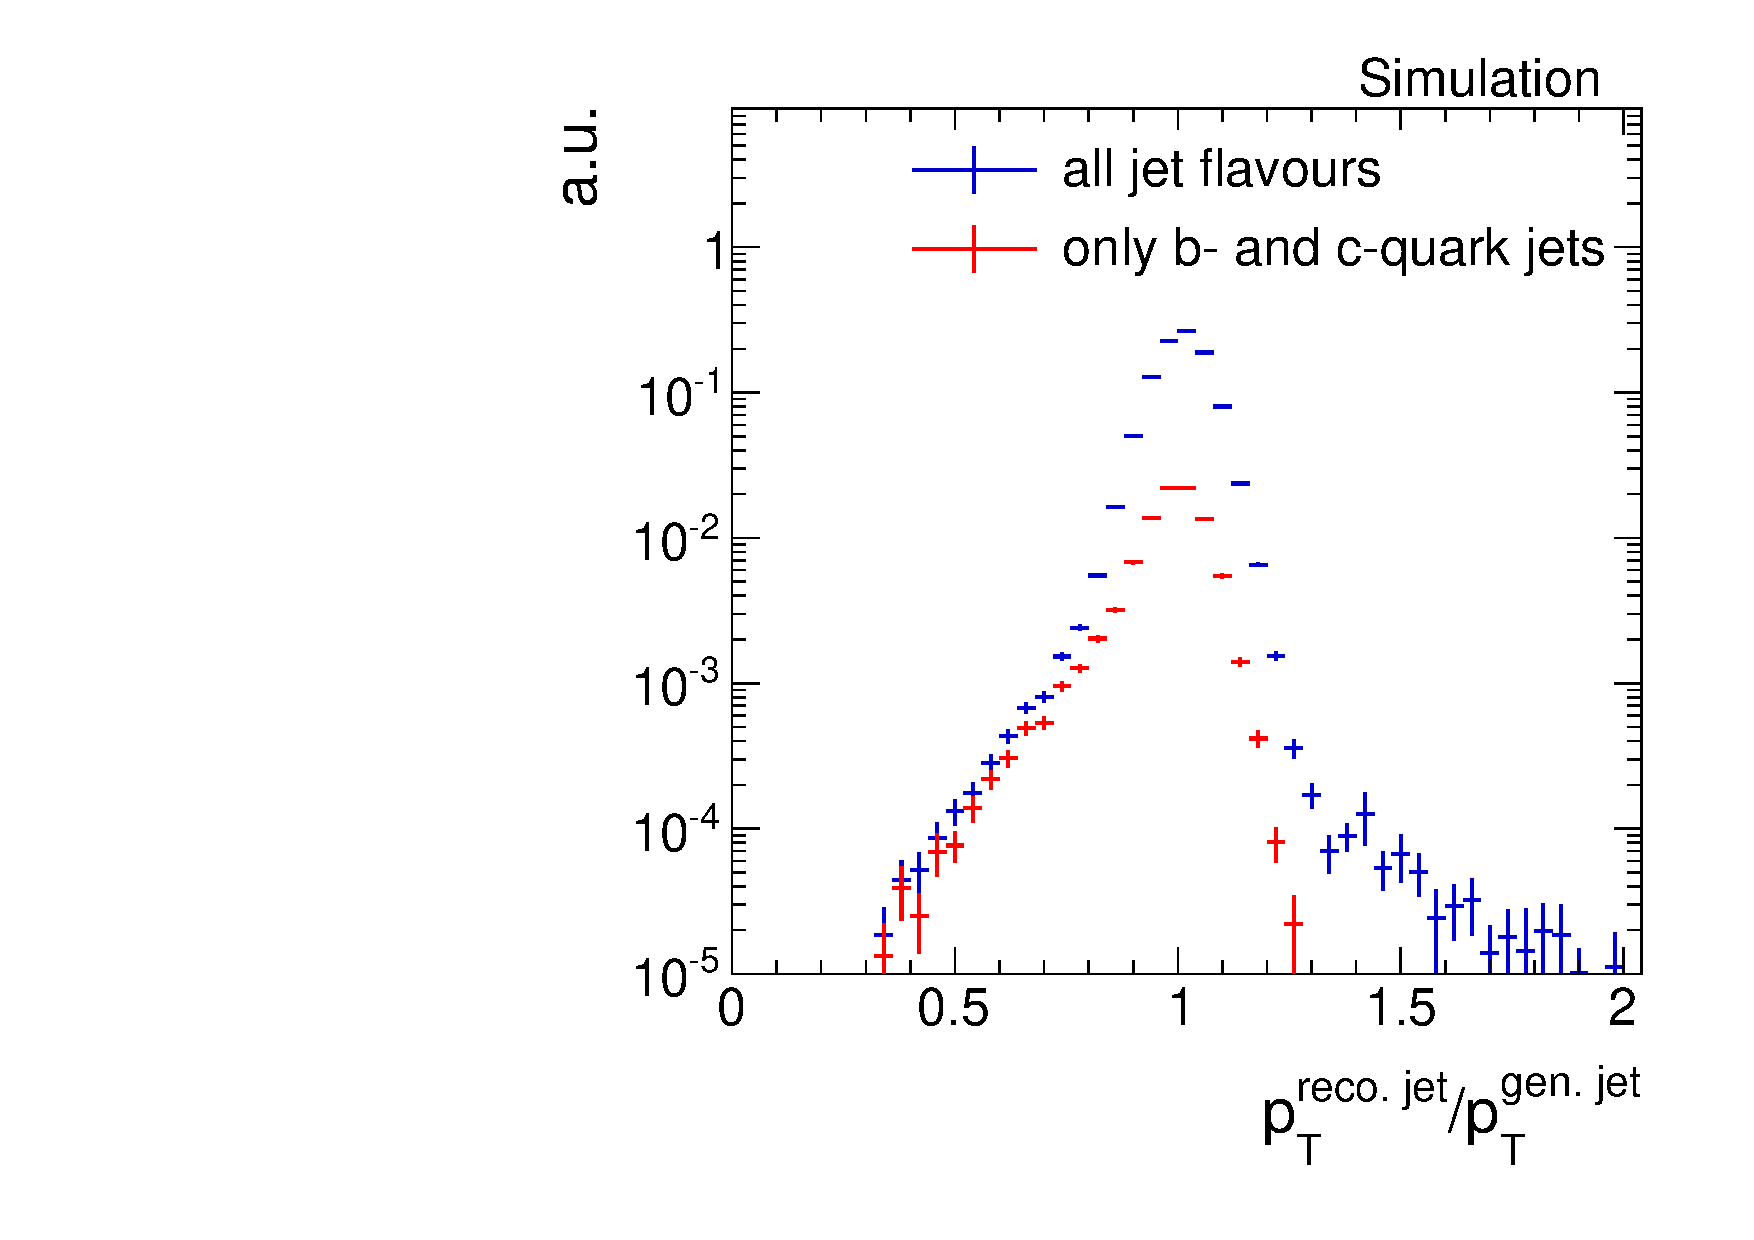
\includegraphics[width=0.49\textwidth]{figures/resolution/generalApproach/intrinsicExampleContributionofBCQuarks.pdf}
  \caption{Number of events over $\frac{\pt^{\text{reco. jet}}}{\pt^{\text{gen. jet}}}$ from a simulated $\GAMJET$ sample. 
           The black dots show the contribution by c- and b-quark jets where the left tail originating from semi-leptonic decays of heavy quarks can be seen.}  
  \label{fig:TypicalResponse}
\end{figure}
The core of the response distribution shows a Gaussian behavior whereas the tails deviate from that functional form.
Physical reasons for the low response tail are inter alia semi-leptonic decays of heavy quarks where the neutrino cannot be detected and the reconstructed transverse momentum of the jet is too small (see \mbox{Fig. \ref{fig:TypicalResponse}}). 
Some instrumental effects, such as a non-linear response of the calorimeter, inhomogeneities of the detector material and electronic noise can contribute to both tails, 
others, like dead calorimeter channels only contribute to the left tail. 
The resolution is therefore determined using only the core of the distribution to avoid the coverage of non-Gaussian tails.

Therefore, in this analysis note the resolution is defined as the standard deviation of the 99\% truncated response histogram devided by the mean of the histogram:

\begin{equation}\label{eq:resolutionFormula}
\text{JER} = \frac{\sigma_{99\%}}{\mu_{99\%}}.
\end{equation}

The determination of the 99\% range of the histogram is done in several steps. 
First the mean of the core is found via a Gaussian fit to the histogram in a 2$\sigma$ range \footnote{The 2$\sigma$ range is defined as the range [$\mu - 2\sigma$,$\mu + 2\sigma$].}. 
This procedure is done in three iteration steps.
Then, a symmetric interval around this mean is determined with its integral equal to 99\% of the integral of the full histogram. 

%The division by the mean is done to make the resolution measurement more insensitive to a variation of the jet energy scale (= mean of the response distribution)
%which has also an effect on the measured width of the distribution. 
%because response distributions with a scale smaller than one are typically narrower while distributions with scales larger than one are broader.

The evaluation of the response distribution as reconstructed over generated jet transverse momentum (\mbox{Eq.~\eqref{eq:responseFormula}})
is only possible for simulated events where generator information is accessible. 
A determination of the resolution in data, however, has to rely on a different approach.

The main idea of a resolution measurement using $\GAMJET$ events is based on the transverse momentum balance of the system and the excellent electromagnetic calorimeter resolution
(which was estimated between 1.1 \% and 2.6\% in the barrel region for photons for $\sqrt{s}= 7 \tev$ data \cite{bib:CMS:ECALresolution_7TeV} 
and is expected to be similar for $\sqrt{s}= 8 \tev$ data).

Several tree-level processes (\mbox{see Fig. \ref{fig:FeynmanDiagrams}}) lead to an event topology with one photon and one jet in the final state. 

\begin{figure}[htp]
  \centering

      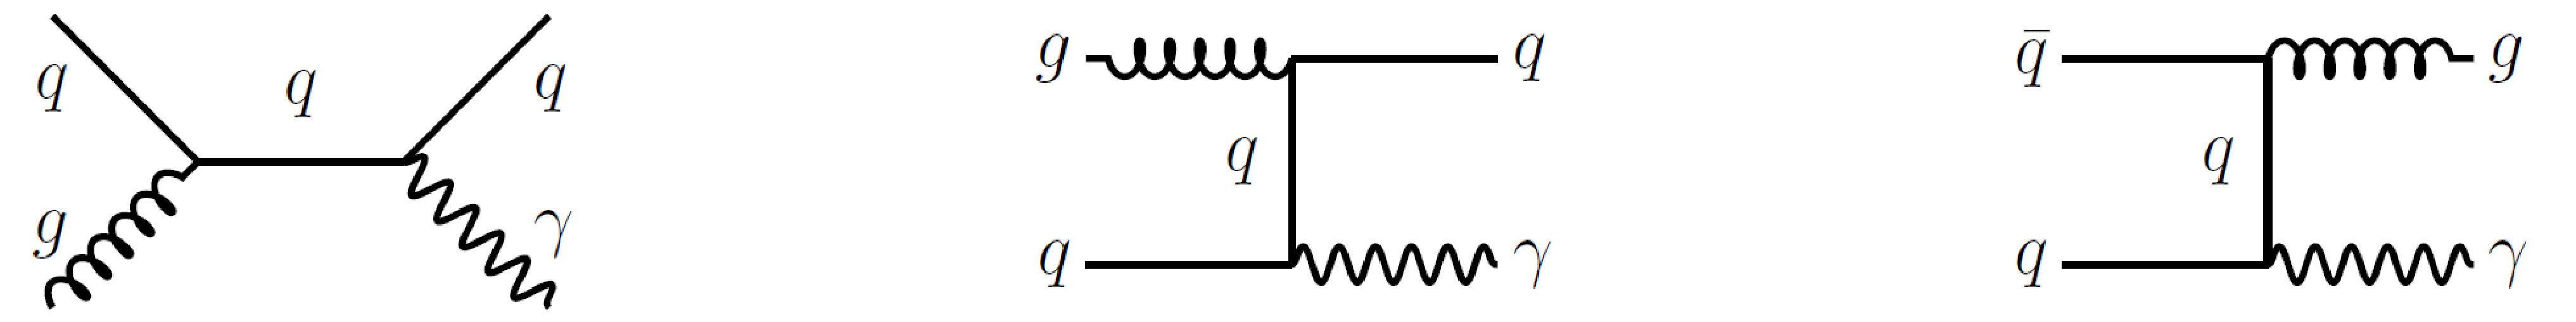
\includegraphics[width=0.99\textwidth]{figures/resolution/generalApproach/FeynmanDiagram.pdf}
 
 
  \caption{Tree-level Feynman diagrams of processes at the LHC in pp collisions with one photon and one jet in the final state.}  
  \label{fig:FeynmanDiagrams}
\end{figure}
Due to momentum conversation, the jet and the photon are back to back in the transverse plane, and therefore, $\vec{p}_{T}^{\gamma} = -\vec{p}_{T}^{\text{jet}}$. 
Because of the good resolution of the electromagnetic calorimeter, photon energies can be very well measured 
and thus can serve as an excellent estimator for the true jet energy.


Unfortunately, such clean events are very rare processes, and usually, the momentum balance is spoiled by initial and final state radiation, which lead to further jets in the event 
(see \mbox{Fig. \ref{fig:FeynmanDiagramsWithRadiation}}). 
However, in order to select events that are balanced to a large extent, a lower bound 
on the angular distance in the transverse plane between the photon and the jet with the highest transverse momentum (leading jet) is required ($\Delta\Phi>2.95\unit{rad}$). 

Additionally, the variable 

\begin{equation}\label{eq:alphaDef}
\alpha \doteq \frac{\pt^{\text{\nth{2} reco. jet}}}{\pt^{\gamma}}
\end{equation} 
is defined as a measure of further jet activity in an event. 
It is, however, not sufficient to require only an upper bound on $\alpha$. 
Instead, the jet energy resolution is measured in bins of $\alpha$ (with max($\alpha$) = 0.2), 
and the \mbox{extrapolated} value to zero further jet energy ($\alpha=0$) is taken as the measured resolution of the jet energy in the absence of further jets.


\begin{figure}[t]
  \centering

      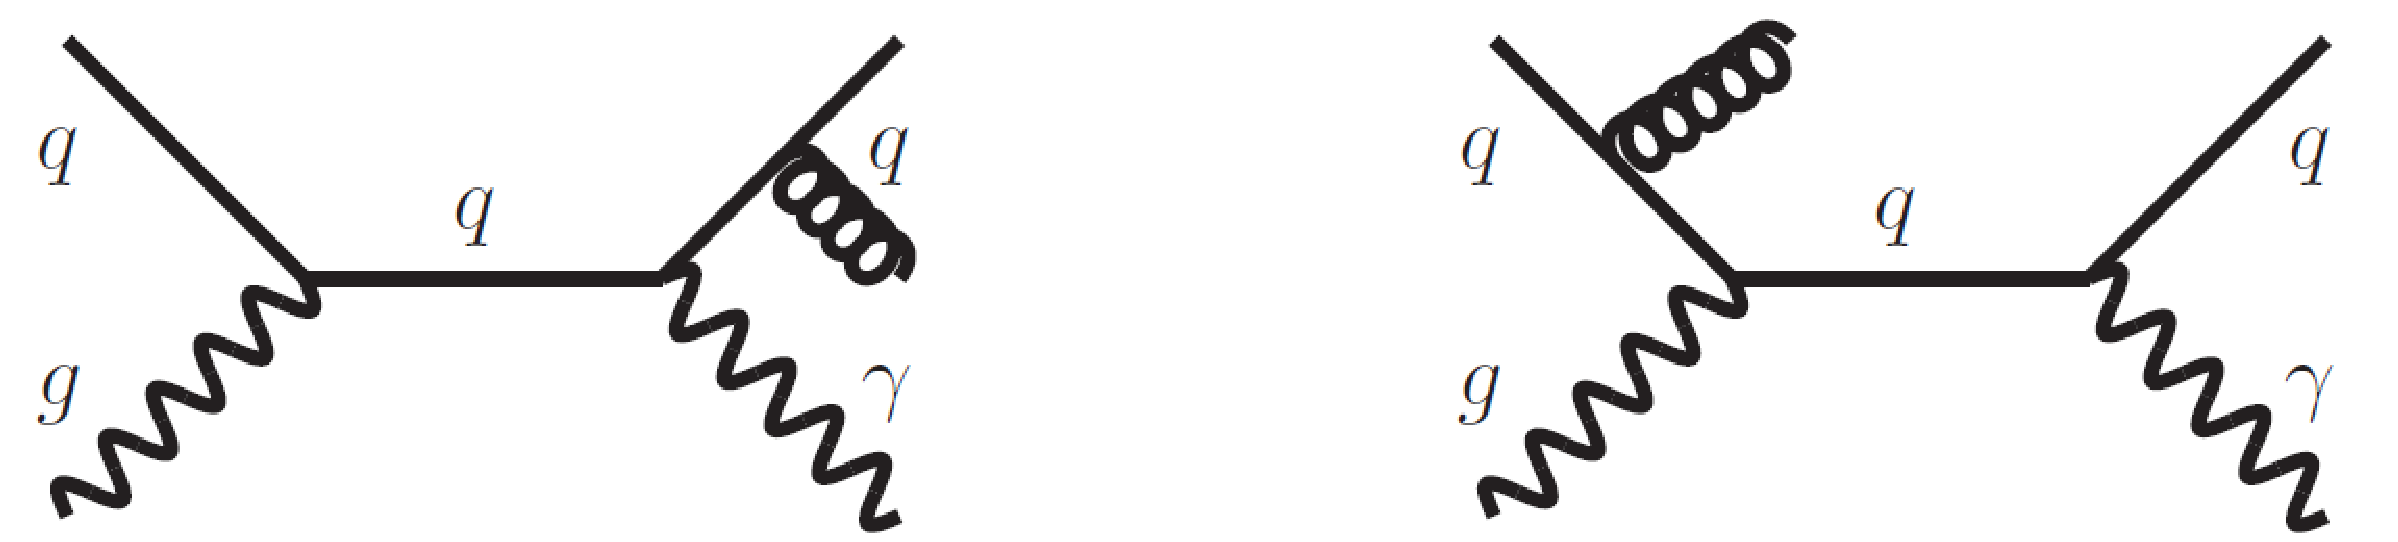
\includegraphics[width=0.60\textwidth]{figures/resolution/generalApproach/FeynmanDiagramsWithRadiation.pdf}
  
  \caption{Tree-level Feynman diagrams with initial and final state radiation.}  
  \label{fig:FeynmanDiagramsWithRadiation}
\end{figure}

Measuring the transverse momentum of the photon instead of taking the generator jet $p_{T}$ leads to the fact that the measured resolution consists out of two parts

\begin{equation}\label{eq:splitting}
\frac{\pt^{\text{reco. jet}}}{\pt^{\gamma}} = \underbrace{\frac{\pt^{\text{reco. jet}}}{\pt^{\text{gen. jet}}}}_{\text{intrinsic}} \cdot \underbrace{\frac{\pt^{\text{gen. jet}}}{\pt^{\gamma}}}_{\text{imbalance}}.
\end{equation}

The intrinsic part is the resolution of interest which is independent of further jets in the event whereas the imbalance is strongly dependent on $\alpha$.

To extract the intrinsic resolution out of the measured one, the residual imbalance $q^{\prime}$ (the imbalance at $\alpha = 0$) is subtracted from the total resolution in the 
limit of vanishing additional jet activity. 
As that information is only available from simulation, the measured resolution in data is corrected by the residual imbalance taken from the simulated data set.
%%%%%%%%%%%%%%%%%%%%%%%%%%%%%%%%%%%%%%%%%%%%%%%%%%%%%%%%%%%%%%%%%%%%%%%%%%%%%%%%%%%%%%%%%%%%%%%%%%%%%%%%%%%%%%%%%%%%%%%%%%%%%%%%%%%%%%%%%%%%%%%%%%%%%%%%%%%%%%%%%%%%%%%%%%%%%%%%%%%%%%%%%%%%%%%%%%%%%%%%%%%%%%%%%%%%%%%%%%%%%%%%%%%%%%%%%%%

%%%%%%%%%%%%%%%%%%%%%%%%%%%%%%%%%%%%%%%%%%%%%%%%%%%%%%%%%%%%%%%%%%%%%%%%%%%%%%%%%%%%%%%%%%%%%%%%%%%%%%%%%%%%%%%%%%%%%%%%%%%%%%%%%%%%%%%%%%%%%%%%%%%%%%%%%%%%%%%%%%%%%%%%%%%%%%%%%%%%%%%%%%%%%%%%%%%%%%%%%%%%%%%%%%%%%%%%%%%%%%%%%%%%%%%%%%%
%%%%%%%%%%%%%%%%%%%%%%%%%%%%%%%%%%%%%%%%%%%%%%%%%%%%%%%%%%%%%%%%%%%%%%%%%%%%%%%%%%%%%%%%%%%%%%%%%%%%%%%%%%%%%%%%%%%%%%%%%%%%%%%%%%%%%%%%%%%%%%%%%%%%%%%%%%%%%%%%%%%%%%%%%%%%%%%%%%%%%%%%%%%%%%%%%%%%%%%%%%%%%%%%%%%%%%%%%%%%%%%%%%%%%%%%%%%
\chapter{Datasets and event selection}

\begin{itemize}
\item  selection - take from AN
\end{itemize}

Pictures as root file available:
\begin{itemize}
\item BLA
\end{itemize}

Picture \textcolor{red}{NOT} as root file available:
\begin{itemize}
\item BLA
\end{itemize}
%%%%%%%%%%%%%%%%%%%%%%%%%%%%%%%%%%%%%%%%%%%%%%%%%%%%%%%%%%%%%%%%%%%%%%%%%%%%%%%%%%%%%%%%%%%%%%%%%%%%%%%%%%%%%%%%%%%%%%%%%%%%%%%%%%%%%%%%%%%%%%%%%%%%%%%%%%%%%%%%%%%%%%%%%%%%%%%%%%%%%%%%%%%%%%%%%%%%%%%%%%%%%%%%%%%%%%%%%%%%%%%%%%%%%%%%%%%

%%%%%%%%%%%%%%%%%%%%%%%%%%%%%%%%%%%%%%%%%%%%%%%%%%%%%%%%%%%%%%%%%%%%%%%%%%%%%%%%%%%%%%%%%%%%%%%%%%%%%%%%%%%%%%%%%%%%%%%%%%%%%%%%%%%%%%%%%%%%%%%%%%%%%%%%%%%%%%%%%%%%%%%%%%%%%%%%%%%%%%%%%%%%%%%%%%%%%%%%%%%%%%%%%%%%%%%%%%%%%%%%%%%%%%%%%%%
%%%%%%%%%%%%%%%%%%%%%%%%%%%%%%%%%%%%%%%%%%%%%%%%%%%%%%%%%%%%%%%%%%%%%%%%%%%%%%%%%%%%%%%%%%%%%%%%%%%%%%%%%%%%%%%%%%%%%%%%%%%%%%%%%%%%%%%%%%%%%%%%%%%%%%%%%%%%%%%%%%%%%%%%%%%%%%%%%%%%%%%%%%%%%%%%%%%%%%%%%%%%%%%%%%%%%%%%%%%%%%%%%%%%%%%%%%%
\chapter{Methodology of the measurement}

\begin{itemize}
\item Take from AN
\end{itemize}

Pictures as root file available:
\begin{itemize}
\item BLA
\end{itemize}

Picture \textcolor{red}{NOT} as root file available:
\begin{itemize}
\item BLA
\end{itemize}
%%%%%%%%%%%%%%%%%%%%%%%%%%%%%%%%%%%%%%%%%%%%%%%%%%%%%%%%%%%%%%%%%%%%%%%%%%%%%%%%%%%%%%%%%%%%%%%%%%%%%%%%%%%%%%%%%%%%%%%%%%%%%%%%%%%%%%%%%%%%%%%%%%%%%%%%%%%%%%%%%%%%%%%%%%%%%%%%%%%%%%%%%%%%%%%%%%%%%%%%%%%%%%%%%%%%%%%%%%%%%%%%%%%%%%%%%%%

%%%%%%%%%%%%%%%%%%%%%%%%%%%%%%%%%%%%%%%%%%%%%%%%%%%%%%%%%%%%%%%%%%%%%%%%%%%%%%%%%%%%%%%%%%%%%%%%%%%%%%%%%%%%%%%%%%%%%%%%%%%%%%%%%%%%%%%%%%%%%%%%%%%%%%%%%%%%%%%%%%%%%%%%%%%%%%%%%%%%%%%%%%%%%%%%%%%%%%%%%%%%%%%%%%%%%%%%%%%%%%%%%%%%%%%%%%%
%%%%%%%%%%%%%%%%%%%%%%%%%%%%%%%%%%%%%%%%%%%%%%%%%%%%%%%%%%%%%%%%%%%%%%%%%%%%%%%%%%%%%%%%%%%%%%%%%%%%%%%%%%%%%%%%%%%%%%%%%%%%%%%%%%%%%%%%%%%%%%%%%%%%%%%%%%%%%%%%%%%%%%%%%%%%%%%%%%%%%%%%%%%%%%%%%%%%%%%%%%%%%%%%%%%%%%%%%%%%%%%%%%%%%%%%%%%
\chapter{Systematic uncertainties}

\begin{itemize}
\item difficult to take from AN
\end{itemize}

Pictures as root file available:
\begin{itemize}
\item BLA
\end{itemize}

Picture \textcolor{red}{NOT} as root file available:
\begin{itemize}
\item BLA
\end{itemize}
%%%%%%%%%%%%%%%%%%%%%%%%%%%%%%%%%%%%%%%%%%%%%%%%%%%%%%%%%%%%%%%%%%%%%%%%%%%%%%%%%%%%%%%%%%%%%%%%%%%%%%%%%%%%%%%%%%%%%%%%%%%%%%%%%%%%%%%%%%%%%%%%%%%%%%%%%%%%%%%%%%%%%%%%%%%%%%%%%%%%%%%%%%%%%%%%%%%%%%%%%%%%%%%%%%%%%%%%%%%%%%%%%%%%%%%%%%%

%%%%%%%%%%%%%%%%%%%%%%%%%%%%%%%%%%%%%%%%%%%%%%%%%%%%%%%%%%%%%%%%%%%%%%%%%%%%%%%%%%%%%%%%%%%%%%%%%%%%%%%%%%%%%%%%%%%%%%%%%%%%%%%%%%%%%%%%%%%%%%%%%%%%%%%%%%%%%%%%%%%%%%%%%%%%%%%%%%%%%%%%%%%%%%%%%%%%%%%%%%%%%%%%%%%%%%%%%%%%%%%%%%%%%%%%%%%
%%%%%%%%%%%%%%%%%%%%%%%%%%%%%%%%%%%%%%%%%%%%%%%%%%%%%%%%%%%%%%%%%%%%%%%%%%%%%%%%%%%%%%%%%%%%%%%%%%%%%%%%%%%%%%%%%%%%%%%%%%%%%%%%%%%%%%%%%%%%%%%%%%%%%%%%%%%%%%%%%%%%%%%%%%%%%%%%%%%%%%%%%%%%%%%%%%%%%%%%%%%%%%%%%%%%%%%%%%%%%%%%%%%%%%%%%%%
\chapter{Results}

\begin{itemize}
\item THINK
\end{itemize}

Pictures as root file available:
\begin{itemize}
\item BLA
\end{itemize}

Picture \textcolor{red}{NOT} as root file available:
\begin{itemize}
\item BLA
\end{itemize}
%%%%%%%%%%%%%%%%%%%%%%%%%%%%%%%%%%%%%%%%%%%%%%%%%%%%%%%%%%%%%%%%%%%%%%%%%%%%%%%%%%%%%%%%%%%%%%%%%%%%%%%%%%%%%%%%%%%%%%%%%%%%%%%%%%%%%%%%%%%%%%%%%%%%%%%%%%%%%%%%%%%%%%%%%%%%%%%%%%%%%%%%%%%%%%%%%%%%%%%%%%%%%%%%%%%%%%%%%%%%%%%%%%%%%%%%%%%

%%%%%%%%%%%%%%%%%%%%%%%%%%%%%%%%%%%%%%%%%%%%%%%%%%%%%%%%%%%%%%%%%%%%%%%%%%%%%%%%%%%%%%%%%%%%%%%%%%%%%%%%%%%%%%%%%%%%%%%%%%%%%%%%%%%%%%%%%%%%%%%%%%%%%%%%%%%%%%%%%%%%%%%%%%%%%%%%%%%%%%%%%%%%%%%%%%%%%%%%%%%%%%%%%%%%%%%%%%%%%%%%%%%%%%%%%%%
%%%%%%%%%%%%%%%%%%%%%%%%%%%%%%%%%%%%%%%%%%%%%%%%%%%%%%%%%%%%%%%%%%%%%%%%%%%%%%%%%%%%%%%%%%%%%%%%%%%%%%%%%%%%%%%%%%%%%%%%%%%%%%%%%%%%%%%%%%%%%%%%%%%%%%%%%%%%%%%%%%%%%%%%%%%%%%%%%%%%%%%%%%%%%%%%%%%%%%%%%%%%%%%%%%%%%%%%%%%%%%%%%%%%%%%%%%%
\chapter{Discussion and conclusion}

\begin{itemize}
\item Repeat results
\item cross-check analysis
\item Outlook
\end{itemize}

Pictures as root file available:
\begin{itemize}
\item BLA
\end{itemize}

Picture \textcolor{red}{NOT} as root file available:
\begin{itemize}
\item BLA
\end{itemize}
